%!TEX encoding = UTF-8

\chapter{Gesture Recognition Model}
\label{chap:gesture_recognition}

This appendix describes a human gesture recognition model for spotting manipulative hand gestures, inspired by statistical techniques from \ac{ASR}.
This model was used in Ch.~\ref{chap:gestures}, as one of the blocks of the system described therein.

In this appendix, we adopt the following \emph{terminology}.
We use the word \emph{uninterrupted} to refer to a sequence without temporal breaks in between (e.g., an uninterrupted sequence of gestures).
We use the word \emph{continuous} to refer to mathematical real number objects (e.g., the continuous probability between~$0$ and~$1$ associated to the output of a gesture recognition algorithm).

This appendix is the subject of the following publication:
\listPublicationsAppendixGestureRecognition

The outline of this appendix is as follows.
Sec.~\ref{sec:gesture_recognition:background} gives the motivation for building a recognizer of hand gestures in cognitive systems, as well as related work from the literature.
Sec.~\ref{sec:gesture_recognition:approach} provides our proposed approach, including different models that were considered for addressing specific issues.
Sec.~\ref{sec:gesture_recognition:results} lists the gesture recognition results, and finally
Sec.~\ref{sec:gesture_recognition:conclusions} contains our conclusions.

\section{Background and Related Work}
\label{sec:gesture_recognition:background}

Gesture recognition is an important area of research in pattern analysis~\cite{aggarwal:2011}, with applications in diverse fields, including biometrics, surveillance, health and assistive technologies, as well as \hci{} \cite{wigdor:2011,rautaray:2015:survey} and \hri{} \cite{waldherr:2000:ar,yang:2007:tro,bauer:2008:ijhr}.

Several approaches have been proposed for allowing users of artificial systems to employ body gestures for expressing feelings and communicating their thoughts, in the fields of \hci{} \cite{wigdor:2011,rautaray:2015:survey} and \hri{} \cite{waldherr:2000:ar,yang:2007:tro,bauer:2008:ijhr}.
In particular, these fields have seen a surge of interest in interfaces whereby users perform sequences of \emph{uninterrupted}~(therefore natural) physical movements with their hands, body and fingers to interact with smartphones, game consoles, kiosks, desktop computer screens and more.
Therefore, it is important to develop pattern analysis techniques suited for recognizing physical gestures and motion in the context of \hr{} collaboration \cite{kanda:2003:ijcai,dragan:2013:hri,dragan:2014:ar,dragan:2015:hri}.

We now overview specific works about gesture recognition.

The nature of human gestures is ambiguous and context-dependent \cite{mcneill:1996,messing:1999,kita:2017:gesture-concept-hp}: there exist many-to-one mappings between gestures and conveyed concepts, making gesture recognition a difficult problem.
In addition, in the action aspect, the same gesture can serve different purposes depending on the acted object: for example, the action of pointing and the action of pressing a button are realized by a similar gesture, but they are distinct because of different affected objects.
As such, the ambiguity in mappings between gestures and concepts is also one-to-many.

Different approaches have been proposed to design automatic gesture recognition systems, both to decide which \emph{features} are salient for recognition~\cite{campbell:1996:features} and which \emph{model} best classifies them.
For a comprehensive reviews of these systems, we refer the reader to \cite{wu:1999:review,mitra:2007:review,keskin:2011:hand}.
In particular, designing a recognizer for dynamic gestures (see footnote~\footref{footnote:static_dynamic_gestures} on p.~\pageref{footnote:static_dynamic_gestures}) poses two main issues:
\begin{enumerate}
\item spatio-temporal variability: the same physical gesture can differ in shape and duration, even for the same gesturer;

\item segmentation: the start and end points of a gesture are difficult to define and identify.
\end{enumerate}

Dynamic gestures are essentially a manifestation of body movement, therefore the \emph{high-level features} to recognize them are also related to motion: positions, velocities, accelerations, angles of body joints (including fingers).
These are the features employed in existing gesture recognition solutions based on machine learning, such as Microsoft Visual Gesture Builder for Kinect\footnote{\url{https://developer.microsoft.com/en-us/windows/kinect}, \\ \url{https://channel9.msdn.com/Blogs/k4wdev}}, or the \ac{GRT}\footnote{\url{http://www.nickgillian.com/grt/}}.

The high-level features described above arise from pre-processing algorithms applied to the raw data captured by vision sensors. We refer to this kind of data and to the associated signal processing techniques as \emph{low-level features}, which are commonly: skin color segmentation, optical flow (the apparent visual motion caused by the relative motion of objects and viewer), \armhand{} tracking in 2D or 3D, full body tracking.

Many gesture recognition systems are designed to work in a controlled environment, or they make strong assumptions:
\begin{itemize}
\item limited and fixed lexicon of permitted gestures;

\item availability of the whole test data sequence to classify (system only works offline);

\item constrained physical space (hands must move only within a certain region of upper body);

\item unnatural interaction (isolated gestures, to be preceded and followed by a relaxed pose lasting several seconds);

\item users must wear hardware tracking devices, which can be impractical and expensive.
\end{itemize}

Our gesture recognition model is loosely inspired by neuroscience in the following sense.
Neuroscience experiments have suggested that the area of the human brain responsible for gesture processing is also employed for speech processing~\cite{xu:2009:pnas}, functioning in fact as a modality-independent semiotic system, connecting meaning to various types of symbols: words, gestures, images, sounds, or objects.
The ability to understand and interpret our peers has also been studied in psychology, focusing on internal simulations and re-enactments of previous experiences~\cite{schillaci:2012:hbu,billing:2016:frobt}.

From Sec.~\ref{sec:motivation:neuro:canonical_and_mirror}, recall that mirror neurons are visuomotor neurons that respond to action and object interaction, both when the agent acts and when it observes the same action performed by others, hence the name ``mirror''.

In applying the mirror neuron theory in robotics, as we and others do~\cite{gazzola:2007:neuroimage,lopes:2009:ab}, an agent can first acquire knowledge by sensing and self-exploring its surrounding environment (see Sec.~\ref{sec:platform:scenario}).
Afterwards, it can employ that learned knowledge to novel observations of another agent~(e.g., a human person) who performs similar physical actions to the ones executed during prior training.
In particular, when the two interacting agents are a caregiver and an infant, the mechanism is called \emph{parental scaffolding}, having been implemented on robots too~\cite{ugur:2015:robotica,ugur:2015:tamd}.
These works tackle a problem that is crucial to~(artificial) imitation: how to map action sequences observed in an external agent to action sequences performed by an imitator agent, which in general may have different affordances and a different body morphology (this issue is also known as the \emph{correspondence problem}~\cite{nehaniv:2002:correspondence}). \label{para:correspondence_problem}
In our case, we consider a simple collaboration scenario and we assume that the two agents are capable of applying actions to objects leading to similar effects, enabling the transfer, and that they operate on a shared space~(i.e., a table accessible by both agents' arms).
The morphology and the motor realization of the actions can be different between the two agents.

Some authors have studied the ability to interpret other agents under the deep learning paradigm.
In~\cite{kim:2017:nn}, a recurrent neural network is proposed to have an artificial simulated agent infer human intention~(as output) from joint input information about objects, their potential affordances or opportunities, and human actions, employing different time scales for different actions.
However, in that work a virtual simulation able to produce large quantities of data was used.
This is both unrealistic when trying to explain human cognition, and limited, because a simulator cannot model all the physical events and the unpredictability of the real world.
In contrast, we use real, noisy data acquired from robots and sensors to validate our model.

We propose that the link between gesture and speech justifies the usage of machinery that, as in \ac{ASR},
is suited for capturing dynamic time series data (i.e., a series of data points, listed in time order, that represent the measurement of some quantity over time).
\acp{HMM}, which we explain in Sec.~\ref{sec:hmm}, are one such statistical tool.
We adopt an \acs{HMM}-based approach to recognize body gestures that follow \emph{temporally dynamic patterns}.

\section{Proposed Approach}
\label{sec:gesture_recognition:approach}

We now describe the design of our human gesture recognition model.

In this section, we present a human action recognition method for manipulative hand gestures, its theory (\aclp{HMM}), properties and training phase, and how to evaluate the tests.

From the beginning of this appendix, recall the online, real-time nature of our approach, which analyzes human gestures uninterruptedly, classifying them statistically.
The set of body gestures which we use consists of grasp, tap, and touch movements\footnote{%
In an earlier version of our gesture recognizer~\cite{saponaro:2013:crhri} we also trained a fourth gesture (touch, shown in Fig.~\ref{fig:gestures:human:touch}), but we later discarded it in order to combine three gestures with the three actions of the pre-existing \AffWords{} system~\cite{salvi:2012:smcb}. In terms of hand kinematics, the touch gesture is identical to the grasp gesture (shown in Fig.~\ref{fig:gestures:human:grasp}), the only difference being that in the former the object is not grasped by the person, whereas in the latter it is grasped. \label{footnote:touch_gesture} % end footnote
}: these gestures pertain to manipulation tasks, and they are shown in Fig.~\ref{fig:gestures:human_action_examples}.

Each of the gestures under consideration is represented by a \ac{HMM}, which we will first define formally in Sec.~\ref{sec:hmm}.
Then, we will present two baseline models and our final model in Sec.~\ref{sec:gesture_recognition:approach:gesture_model:models}: these are models of increasing complexity and power, for combining the gesture \acp{HMM} together, permitting loops of gestures, and to treat noise information (i.e., the transition frames between two consecutive gestures) appropriately.

\subsection{\aclp{HMM}}
\label{sec:hmm}

\acp{HMM}~\cite{rabiner:1989:hmm} are a statistical tool for modeling time series data. They have been applied to the segmentation and recognition of sequential data with spatial and temporal variability such as speech, machine translation, genomics, financial data, among others.
One of the advantages of \acp{HMM}, and a reason behind their popularity, is the fact that they are computationally tractable thanks to dynamic programming techniques: marginal probabilities and samples can be obtained from an \ac{HMM} with the \FB{} algorithm~\cite[Sec.~III.A]{rabiner:1989:hmm}, and the most likely sequence of hidden states can be estimated with the \Viterbi{} algorithm~\cite[Sec.~III.B]{rabiner:1989:hmm}.

An \ac{HMM} with continuous outputs is defined by a set of discrete states~$\mathcal{S} = \{s_1, \dots, s_Q\}$ and by a set of parameters $\lambda = \{ A, B, \Pi \}$, where $A = \{ a_{ij} \}$ is the transition probability matrix, $a_{ij}$ is the transition probability from state~$s_i$ at time~$t$ to state~$s_j$ at time~$t+1$, $B = \{ f_i \}$ is the set of $Q$~observation probability functions (one per state~$i$) with continuous values (typically mixture-of-Gaussians \aclp{PDF}), and $\Pi$ is the initial probability distribution for the states.

In our case, the model for each action is a left-to-right \ac{HMM}, where the transition model between the~$Q$ discrete states~$\mathcal{S} = \{s_1, \dots, s_Q\}$ is structured so that states with a lower index represent events that occur earlier in time.

The continuous variables~$g_i$ are measured at regular time intervals.
At a certain time step~$t$, the $D$-dimensional feature vector can be expressed as~$\bm{g}[t] = \{g_1[t], \dots, g_D[t]\}$.
The input to the model is a sequence of~$T$ such feature vectors~$\bm{g}[1], \dots, \bm{g}[T]$ that we call for simplicity~$G_1^T$, where~$T$ can vary for every recording.

At recognition~(testing) time, we can use the models to estimate the likelihood of a new sequence of observations~$G_1^T$ given each possible action, by means of the \FB{} inference algorithm.
We can express this likelihood as $\mathcal{L}_\text{HMM}(G_1^T \given A=a_k)$, where $a_k$ is one of the possible actions of Fig.~\ref{fig:gestures:human_action_examples}.
By normalizing the likelihoods, assuming that the gestures are equally likely \apriori, we can obtain the posterior probability of the action given the sequence of observations (see Sec.~\ref{sec:background:theory:probability} for an explanation of Bayesian inference) as
\begin{equation} \label{eq:phmm_action}
  \phmm(A=a_k \given G_1^T) = \frac{\mathcal{L}_\text{HMM}(G_1^T \given A=a_k)}{\sum_h \mathcal{L}_\text{HMM}(G_1^T \given A=a_h)}.
\end{equation}

\subsection{Baseline Models and Final Model}
\label{sec:gesture_recognition:approach:gesture_model:models}

We propose and compare three different models to recognize dynamic human gestures, with increasing complexity and expressive power for combining the gesture \acp{HMM} together with noise information.
These are two baseline models (Model~1, Model~2) and our final model (Model~3).
Model~3 is the one that permits uninterrupted gesture recognition, loops of gestures, and also to treat noise information (i.e., the transition frames between two consecutive gestures) appropriately.

All of the three models are composed by a set of \acp{HMM} (one for each dynamic human gesture), and an additional \ac{HMM} for modeling noise.
By noise we refer to \emph{nongesture} data points, also known as \emph{garbage} in the \ac{ASR} literature.
Depending on the model, these garbage points will be represented either with a single-state \ac{HMM}, or with a multi-state \ac{HMM}.
Each state of all our \acp{HMM} emits a mixture of Gaussians as output, also known as \ac{GMM}.
By \ac{GMM} we mean a linear superposition of components with Gaussian densities (a \ac{GMM} can be thought as a single-state \ac{HMM}).

\newcommand{\myscalefactor}{0.8}

\newcommand{\standardhmm}[1]{
    \node[draw,circle] (hmm#1s1) {1};
    \node[draw,circle, right of=hmm#1s1] (hmm#1s2) {2};
    \node[circle, right of=hmm#1s2] (hmm#1s3) {\dots};
    \node[draw,circle, right of=hmm#1s3] (hmm#1s4) {Q};
    \node[left of=hmm#1s1]  (invisible1) {};
    \node[right of=hmm#1s4] (invisible2) {};
    \path[->] (hmm#1s1) edge (hmm#1s2);
    \path[loop above] (hmm#1s1) edge (hmm#1s1);
    \path[->] (hmm#1s2) edge (hmm#1s3);
    \path[loop above] (hmm#1s2) edge (hmm#1s2);
    \path[dashed] (hmm#1s2) -- (hmm#1s3);
    \path[->] (hmm#1s3) edge (hmm#1s4);
    \path[loop above] (hmm#1s4) edge (hmm#1s4);
    \path[->] (invisible1) edge (hmm#1s1);
    \path[->] (hmm#1s4) edge (invisible2);
}

\newcommand{\modelone}{
    \begin{tikzpicture}[scale=\myscalefactor, every node/.style={scale=\myscalefactor}]
      \matrix (M) [matrix of nodes, ampersand replacement=\&] {%
      hmm1 \& \standardhmm{1} \\
      hmm2 \& \standardhmm{2} \\
      hmm3 \& \standardhmm{3} \\
      garbage
      \& %
      \node[draw,circle] (gmm_node) {1};
      \node[left of=gmm_node]  (invisible1) {};
      \node[right of=gmm_node] (invisible2) {};
      \path[->] (invisible1) edge (gmm_node);
      \path[->] (gmm_node) edge (invisible2);
      \path[loop above] (gmm_node) edge (gmm_node); \\
      };
    \end{tikzpicture}
}

\newcommand{\modelonegest}{
    \begin{tikzpicture}[scale=\myscalefactor, every node/.style={scale=\myscalefactor}]
      \node[draw,circle] (hmm1s1) {1};
      \node[draw,circle, right of=hmm1s1] (hmm1s2) {2};
      \node[circle, right of=hmm1s2] (hmm1s3) {\dots};
      \node[draw,circle, right of=hmm1s3] (hmm1s4) {Q};
      \node[left of=hmm1s1]  (invisible1) {};
      \node[right of=hmm1s4] (invisible2) {};
      \path[->] (hmm1s1) edge (hmm1s2);
      \path[loop above] (hmm1s1) edge (hmm1s1);
      \path[->] (hmm1s2) edge (hmm1s3);
      \path[loop above] (hmm1s2) edge (hmm1s2);
      \path[dashed] (hmm1s2) -- (hmm1s3);
      \path[->] (hmm1s3) edge (hmm1s4);
      \path[loop above] (hmm1s4) edge (hmm1s4);
      \path[->] (invisible1) edge (hmm1s1);
      \path[->] (hmm1s4) edge (invisible2);
    \end{tikzpicture}
}

\newcommand{\modeltwo}{
  \begin{tikzpicture}[scale=\myscalefactor, every node/.style={scale=\myscalefactor}]
  \matrix (M) [matrix of nodes, ampersand replacement=\&] {%
    hmm1 \& \standardhmm{1} \\
    hmm2 \& \standardhmm{2} \\
    hmm3 \& \standardhmm{3} \\
    garbage \& \standardhmm{4} \\
  };
  \end{tikzpicture}
}

\newcommand{\modelthree}{
  \begin{tikzpicture}[scale=\myscalefactor, every node/.style={scale=\myscalefactor}]
    \node[matrix of nodes, row sep=0.3cm, minimum width=2.5cm] {
      \node[rectangle,draw,fill=red!10] (g1) {gesture1 (tap)}; \\
      \node[rectangle,draw,fill=green!10] (g2) {gesture2 (grasp)}; \\
      \node[rectangle,draw,fill=blue!10] (g3) {gesture3 (push)}; \\
      \node[rectangle,draw] (ga) {garbage}; \\
    };

    \node[circle,draw,left=of g2] (begin) {};
    \node[circle,draw,right=of g2] (end) {};
    \path[->] (begin) edge (g1.west)
              (begin) edge (g2.west)
              (begin) edge (g3.west)
              (begin) edge (ga.west);
    \path[->] (g1.east) edge (end)
              (g2.east) edge (end)
              (g3.east) edge (end)
              (ga.east) edge (end);
    \path[->] (end) edge [bend right=75] (begin);
  \end{tikzpicture}
}

\begin{figure*}
\centering
\subfloat[][Model~1.]
{
   \modelone
   \label{fig:gestures:gesture_models:gmmhmm}
}
%
\subfloat[][Model~2.]
{
  \modeltwo
\label{fig:gestures:gesture_models:hmms} }
\\ %
\subfloat[][Model~3.]
{
  \modelthree
  \label{fig:gestures:gesture_models:hmms_combined}
}
%
\caption[Different \acl{HMM} structures considered when developing our gesture recognizer.]{Different \acl{HMM} structures considered when developing our gesture recognizer. Every state is associated to an emission \acl{PDF} which is a mixture of Gaussians. \\%
Model~1: one multi-state \ac{HMM} per human gesture, one single-state \ac{HMM} (i.e., a \ac{GMM} without transitions) for garbage data. Each model in~$\{\text{hmm1, hmm2, hmm3}\}$ is independent from the other ones and can have an arbitrary number of states. \\%
Model~2: one multi-state \ac{HMM} per human gesture, one multi-state \ac{HMM} for garbage data. Each model in~$\{\text{hmm1, hmm2, hmm3, garbage}\}$ is independent from the other ones and can have an arbitrary number of states \\%
Model~3. one multi-state \ac{HMM} per human gesture, one multi-state \ac{HMM} for garbage data. These four configurations are then merged with an outer transition loop. Each rectangle represents a gestural \ac{HMM} like the ones shown in Fig.~\ref{fig:gestures:gesture_models:hmms}, however, because of the merging, the original state indexes of~$\{\text{hmm1, hmm2, hmm3, garbage}\}$ must be now uniquely renumbered.}
\label{fig:gestures:gesture_models}
\end{figure*}

Having established that all of the models are characterized by multi-state \acp{HMM}, one for each gesture, let us explain the main difference among the three models with respect to the \emph{garbage} representation.
The three different graphical models, represented in Fig.~\ref{fig:gestures:gesture_models}, are:
\begin{itemize}
\item Model~1: the garbage is modeled as a single-state \ac{HMM} (therefore it coincides with a simple \ac{GMM} without temporal transitions). In the experimental part (see Sec.~\ref{sec:gesture_recognition:results}) we will see how this model is not able to represent transitions during nongesture phases;

\item Model~2: the garbage is modeled as a multi-state \ac{HMM}, thus providing a richer representation able to capture nongesture transitions. However, after a gesture is done being recognized, this model does not permit to recognize another gesture (absence of transitions between gestures);

\item Model~3: like the previous one, in addition transitions between gestures are allowed. This permits us to finally capture the uninterrupted aspect of natural human gesture sequences.
\end{itemize}

\subsection{Feature Selection}
\label{sec:gesture_recognition:approach:gesture_model:features}

The features that we use to train our gesture classifier are the spatial 3D coordinates of a human's hand joint being tracked\footnote{%
It is possible to use more joints as features, for example the concatenation of hands, elbows, shoulders, torso and head coordinates, as mentioned in Sec.~\ref{sec:gesture_recognition:background}. In our domain, data, and tests, using just the hand joint features yielded the highest performance.% end footnote
}, and they can be calculated online without having to wait for an input sequence to be finished.
For this reason, we perform no normalization or filtering that requires knowledge of the completed sequence (e.g., global minima and maxima).
The 3D joints coordinates can be obtained with general-purpose depth cameras like the Microsoft Kinect or the Asus Xtion Pro.
Fig.~\ref{fig:gestures:human_overlay} illustrates the idea of a time series of 3D coordinate features from a dynamic gesture.

\begin{figure}
\centering
\subfloat[][RGB view. Hand trajectory shown in green, elbow trajectory in red.]
{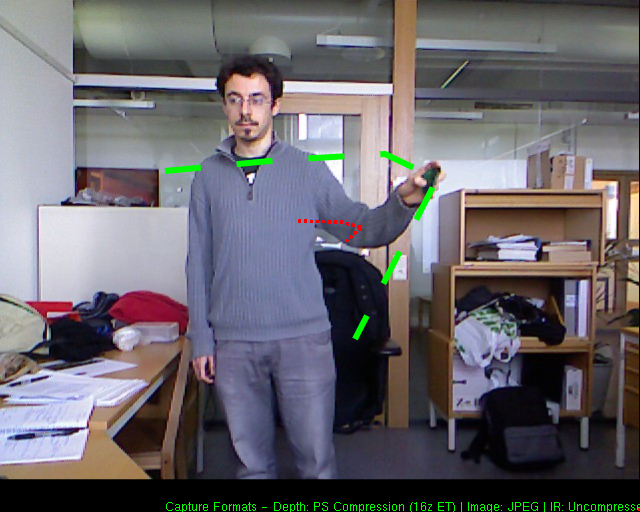
\includegraphics[width=0.41\textwidth]{gesture_recognition_relax-image}
\label{fig:gestures:human_overlay:rgb} } \quad
%
\subfloat[][Depth skeletal view. Hand trajectory shown in green, elbow trajectory in light blue.]
{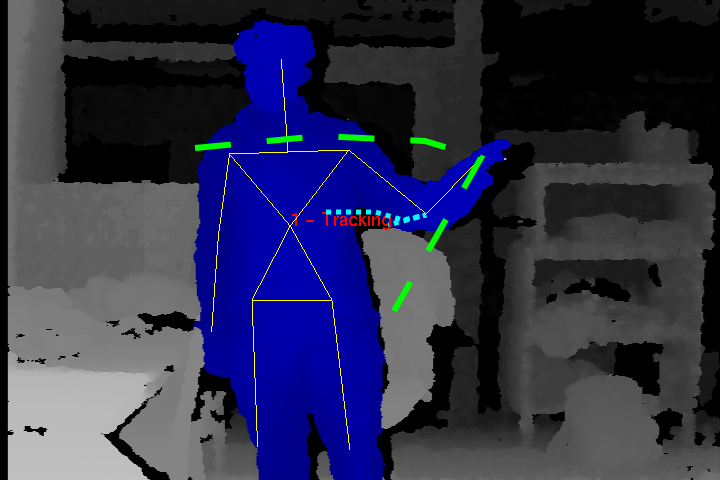
\includegraphics[width=0.49\textwidth]{gesture_recognition_relax-depth}
\label{fig:gestures:human_overlay:d} } \quad
%
\caption[A \emph{tap} human gesture, with temporal trajectory of selected joints being highlighted.]{A \emph{tap} human gesture, with temporal trajectory of selected joints being highlighted. The 3D coordinates of the joints of interest constitute the inputs of our statistical models of Fig.~\ref{fig:gestures:gesture_models}.}
\label{fig:gestures:human_overlay}
\end{figure}

For the simple one-hand actions that we consider as in Fig.~\ref{fig:gestures:human_action_examples}, tracking one hand/arm is sufficient.
While we do not apply normalization steps to the coordinates, we do apply a geometric transformation to the coordinates obtained with depth cameras and skeleton recognition algorithms: we set our reference frame to be \emph{recentered on the human torso}, instead of the default sensor-centered reference frame\footnote{%
The orientation is kept with respect to the camera, because (i)~we focus on frontal person views, not sideways views; (ii)~we will not use orientation features but only positional ones.% end footnote
}.
This transformation has two motivations, a conceptual and a practical one.
Conceptually, it gives more importance to the human user, by placing a virtual mobile point attached to the human user, instead of relying on a fixed point attached to a camera.
From a practical perspective, this transformation provides \emph{invariance to starting point} of a physical gesture. In other words, the user can perform actions at any distance or angle from the sensor, and these actions will always be measured with regards to his torso coordinate.

\subsection{Training}

Following the notation of the \ac{HMM} MATLAB toolbox by Kevin Murphy~\cite{murphy:2012:mlprob}, we introduce the following quantities relative to mixtures of Gaussians, also known as \acp{GMM}. A mixture of~$M$ Gaussian components is the weighted sum of multivariate Gaussian distributions~$m=1,\dots,M$, each with mean~$\mu_m$ and covariance~$\Sigma_m$:
\begin{equation} \label{eq:gmm}
p(x \given w_m, \mu_m, \Sigma_m) = \sum_{m=1}^M w_m \, \mathcal{N}(x \given \mu_m, \Sigma_m),
\end{equation}
where~$x$ is a data point (in our case the 3D hand coordinates), and~$w_m$ are the mixing weights satisfying~$0 \leq w_m \leq 1$,~$\sum_{m=1}^M w_m = 1$.

In addition, for an \ac{HMM} with~$Q$ temporal states we define a \emph{weights matrix} containing all the~$w_m$ as follows: each row represents a state~$q = 1, \dots, Q$, each column represents a mixture component~$m = 1, \dots, M$.

Let~$O$ be the size of an observation vector (e.g., the length of a sequence that we wish to fit to the model during training, or to classify during testing: a segment of~$O$ hand input data points).
Then, we define the \emph{means matrix} with size~$Q \times O M$ to contain the~$\mu_m^{(q)}$ associated to each state~$q$, observed points and mixture components.
Finally, we define a \emph{covariance matrix} with size~$O Q \times O M$ to contain all the~$\Sigma_m^{(q)}$ for each state, observed point and mixture component.

\begin{algorithm}
  \begin{algorithmic} [1]
  \Procedure{UpMix}{weights matrix, means matrix, covariance matrix, $\Mdes$}
  \While{$M$ < $\Mdes$} \Comment{$M$: current no. of Gaussians}
    \State weights: split heaviest entry in two parts with equal weight
    \State means: duplicate corresponding entry
    \State means: perturb new entries to be
    \NoNumber{$\text{means}_{1,2}(i) \, \pm \! = \sqrt{\cov(i,i)} \cdot \text{pertDepth}$}
    \State covariances: duplicate corresponding entry
    \State $M \, := M+1$
  \EndWhile
  \EndProcedure
  \end{algorithmic}
\caption[Gaussian mixture splitting.]{Gaussian mixture splitting. $\Mdes$ is the final desired number of Gaussians; pertDepth is a perturbation depth constant (we set it to $0.2$).} \label{algo:upmix}
\end{algorithm}

For the models described in the remainder of this section, we collected \emph{training data} of one person performing actions without manipulated objects, in other words we trained the gesture recognizer with gesture \emph{pantomimes}.
Each action was performed in \emph{three different amplitudes}: wide gestures (emphatic arm movements), medium-width gestures and narrow gestures (subtle movements).
Each amplitude class was acquired multiple times ($12$--$14$ times), thus providing around $40$~training repetitions for each of the manipulation actions considered.
We show examples of our dataset, with the different amplitudes, in Figs.~\ref{fig:gestures:human:grasp}, \ref{fig:gestures:human:tap}, \ref{fig:gestures:human:push}.

\begin{figure*}
  \centering
  \subfloat{
    \resizebox{\linewidth}{!}{
      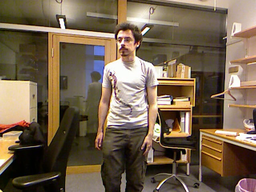
\includegraphics{grasp-wide-img-0022}
      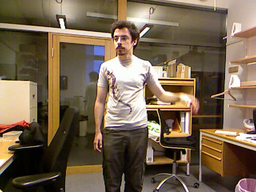
\includegraphics{grasp-wide-img-0023}
      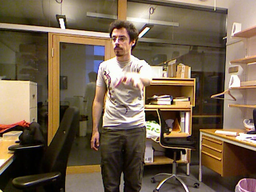
\includegraphics{grasp-wide-img-0024}
      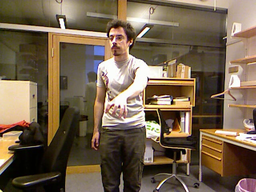
\includegraphics{grasp-wide-img-0025}
      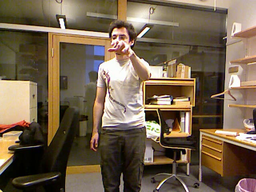
\includegraphics{grasp-wide-img-0027}
      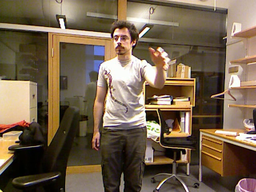
\includegraphics{grasp-wide-img-0029}
    } % end resizebox
  } % end subfloat

  \subfloat{
    \resizebox{\linewidth}{!}{
      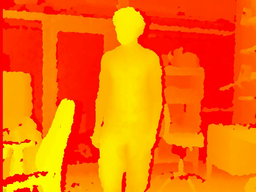
\includegraphics{grasp-wide-depth-0022}
      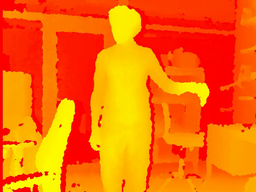
\includegraphics{grasp-wide-depth-0023}
      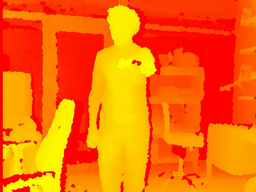
\includegraphics{grasp-wide-depth-0024}
      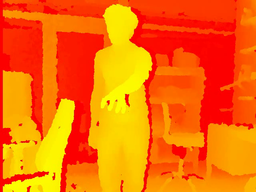
\includegraphics{grasp-wide-depth-0025}
      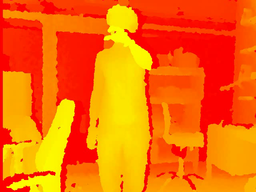
\includegraphics{grasp-wide-depth-0027}
      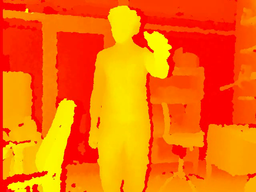
\includegraphics{grasp-wide-depth-0029}
    } % end resizebox
  } % end subfloat

\caption[Gesture recognition data: example sequence of the \emph{grasp} human gesture.]{Gesture recognition data: example sequence of the \emph{grasp} human gesture. Top: image frames, bottom: depth frames. Amplitude: wide, recording number:~2.}
\label{fig:gestures:human:grasp}
\end{figure*}

\begin{figure*}
  \centering
  \subfloat{
    \resizebox{\linewidth}{!}{
      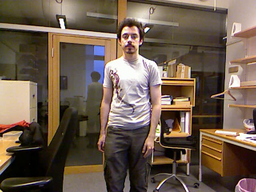
\includegraphics{tap-medium-img-0033}
      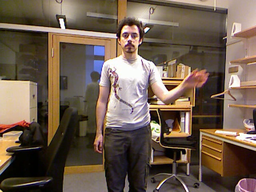
\includegraphics{tap-medium-img-0034}
      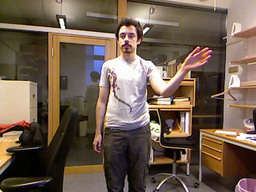
\includegraphics{tap-medium-img-0035}
      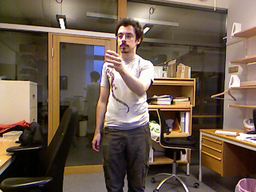
\includegraphics{tap-medium-img-0036}
      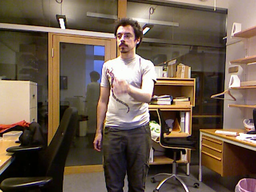
\includegraphics{tap-medium-img-0037}
      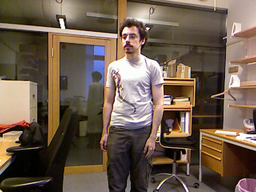
\includegraphics{tap-medium-img-0038}
    } % end resizebox
  } % end subfloat

  \subfloat{
    \resizebox{\linewidth}{!}{
      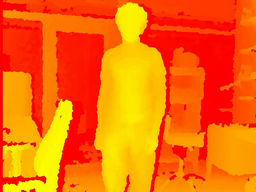
\includegraphics{tap-medium-depth-0033}
      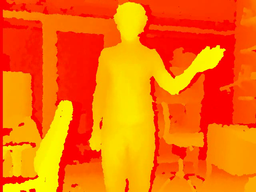
\includegraphics{tap-medium-depth-0034}
      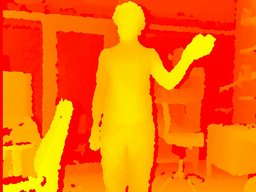
\includegraphics{tap-medium-depth-0035}
      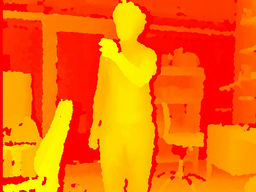
\includegraphics{tap-medium-depth-0036}
      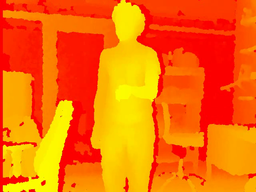
\includegraphics{tap-medium-depth-0037}
      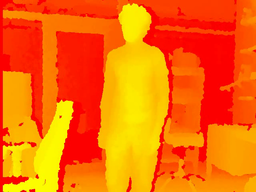
\includegraphics{tap-medium-depth-0038}
    } % end resizebox
  } % end subfloat

\caption[Gesture recognition data: example sequence of the \emph{tap} human gesture.]{Gesture recognition data: example sequence of the \emph{tap} human gesture. Top: image frames, bottom: depth frames. Amplitude: medium, recording number:~4.}
\label{fig:gestures:human:tap}
\end{figure*}

\begin{figure*}
  \centering
  \subfloat{
    \resizebox{\linewidth}{!}{
      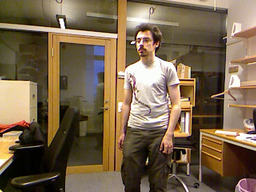
\includegraphics{push-narrow-img-0051}
      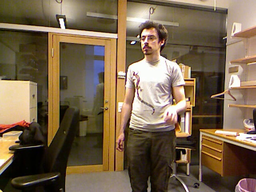
\includegraphics{push-narrow-img-0052}
      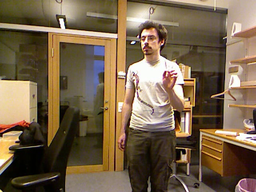
\includegraphics{push-narrow-img-0053}
      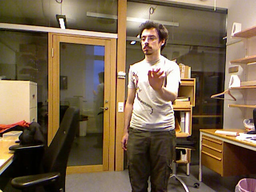
\includegraphics{push-narrow-img-0054}
      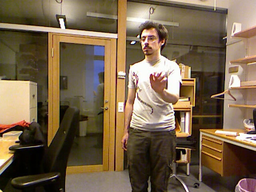
\includegraphics{push-narrow-img-0055}
      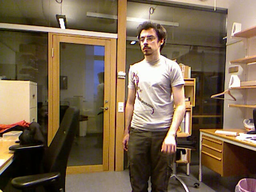
\includegraphics{push-narrow-img-0056}
    } % end resizebox
  } % end subfloat

  \subfloat{
    \resizebox{\linewidth}{!}{
      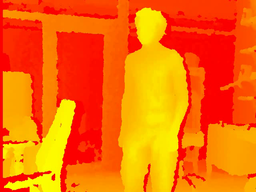
\includegraphics{push-narrow-depth-0051}
      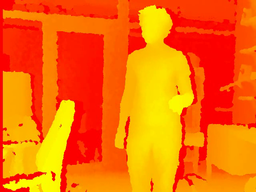
\includegraphics{push-narrow-depth-0052}
      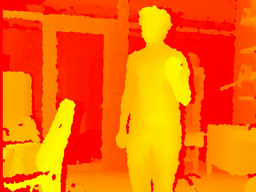
\includegraphics{push-narrow-depth-0053}
      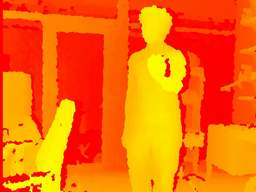
\includegraphics{push-narrow-depth-0054}
      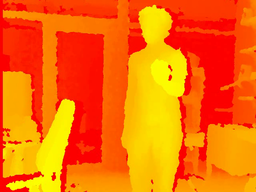
\includegraphics{push-narrow-depth-0055}
      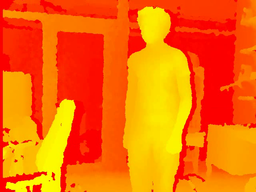
\includegraphics{push-narrow-depth-0056}
    } % end resizebox
  } % end subfloat

\caption[Gesture recognition data: example sequence of the \emph{push} human gesture.]{Gesture recognition data: example sequence of the \emph{push} human gesture. Top: image frames, bottom: depth frames. Amplitude: narrow, recording number:~6.}
\label{fig:gestures:human:push}
\end{figure*}

\begin{figure*}
  \centering
  \subfloat{
    \resizebox{\linewidth}{!}{
      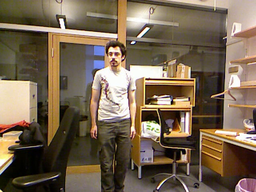
\includegraphics{touch-wide-img-0028}
      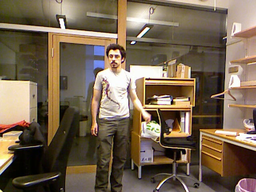
\includegraphics{touch-wide-img-0029}
      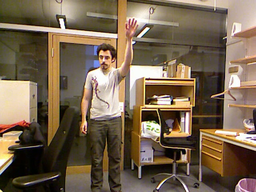
\includegraphics{touch-wide-img-0030}
      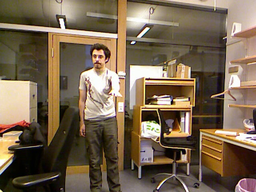
\includegraphics{touch-wide-img-0031}
      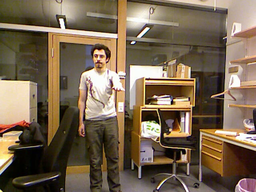
\includegraphics{touch-wide-img-0032}
      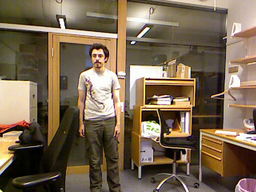
\includegraphics{touch-wide-img-0033}
    } % end resizebox
  } % end subfloat

  \subfloat{
    \resizebox{\linewidth}{!}{
      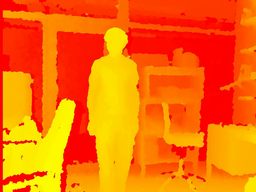
\includegraphics{touch-wide-depth-0028}
      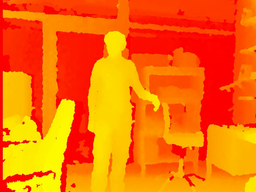
\includegraphics{touch-wide-depth-0029}
      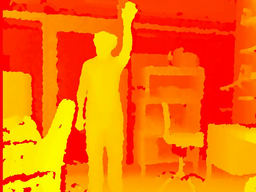
\includegraphics{touch-wide-depth-0030}
      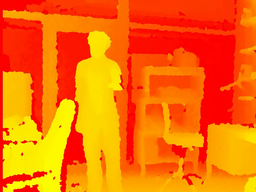
\includegraphics{touch-wide-depth-0031}
      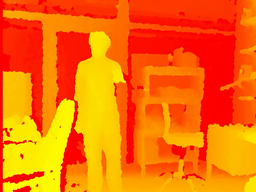
\includegraphics{touch-wide-depth-0032}
      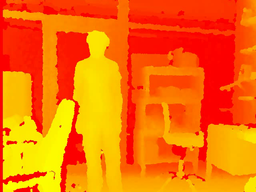
\includegraphics{touch-wide-depth-0033}
    } % end resizebox
  } % end subfloat

\caption[Gesture recognition data: example sequence of the \emph{touch} human gesture.]{Gesture recognition data: example sequence of the \emph{touch} human gesture (see also footnote~\footref{footnote:touch_gesture} on p.~\pageref{footnote:touch_gesture}). Top: image frames, bottom: depth frames. Amplitude: wide, recording number:~3.}
\label{fig:gestures:human:touch}
\end{figure*}

This dataset was used to train all the statistical models described in this section, and we empirically determined suitable initialization characteristics and meta-parameters for our \ac{HMM}:
\begin{itemize}
\item left-to-right \ac{HMM} transition probability matrix (initially every state can either transition to itself or to the next state with equal probability -- with the exception of the last state which only transitions to itself):
      \begin{equation*}
      A = \begin{bmatrix}
          0.5    & 0.5   & 0      & \cdots & 0 \\
          0      & 0.5   & 0.5    & 0      & \vdots \\
          \vdots & \dots & \ddots & \dots  & \vdots \\
          0      & \dots & 0      & 0.5   & 0.5 \\
          0      & \dots & \dots  & 0     & 1
          \end{bmatrix};
      \end{equation*}

\item state probability distribution (initially we impose that we start from the first state, all others having zero probability of starting):
      \begin{equation*}
      \Pi = \begin{bmatrix}1 & 0 & \cdots & 0\end{bmatrix}^{\T}.
      \end{equation*}
\end{itemize}

In all of the models described below, \acp{HMM} were trained with the incremental \emph{mixture splitting} technique, commonly used in \ac{ASR}\footnote{%
However, in recent years, several research groups in the \ac{ASR} community have adopted approaches based on deep neural networks~\cite{hinton:2012:dnn_asr}, rather than on \acp{HMM}.% end footnote
}, in order to obtain the desired number of output Gaussians~$\Mdes$.
With this approach,
initially every mixture has $M=1$~Gaussian (with mean initialized to empirical mean and covariance initialized to empirical covariance of the input data, respectively);
we run the \BW{} algorithm\footnote{The \BW{} algorithm is an instance of the \ac{EM} algorithm used to estimate \ac{HMM} parameters: in our case the weights matrix, the means matrix and the covariance matrix.} to improve \ac{HMM} parameter estimates;
then we enter a cycle, in which we run \UpMix\, (adapted from~\cite[Sec.~10.6]{young:htkbook}, sketched in Alg.~\ref{algo:upmix}) and \BW, increasing the counter~$M$;
the cycle terminates when the weights matrix contains $\Mdes$~Gaussians as desired. This technique allows us to achieve higher likelihoods than with simple \BW~(\EM), as shown in Fig.~\ref{fig:gestures:loglik}.

The first statistical model that we define as a baseline for our experiments (Model~1, shown in Fig.~\ref{fig:gestures:gesture_models:gmmhmm}) consists of several multi-state \acp{HMM} with continuous outputs, one per gesture, and one single-state \ac{HMM} with continuous outputs (i.e., a \ac{GMM}) for garbage.
We use the latter to capture the \emph{noise} (i.e., \emph{nongesture} points), and we use the multi-state \acp{HMM} to model the actual human gestures: each \ac{HMM} is trained for one gesture (many repetitions of the same gesture with different spatial amplitudes and speed).
However, the single-state nature of the garbage model does not allow to capture the dynamic nature which is present in the noisy transitions between subsequent gestures in an uninterrupted, spontaneous human sequence of hand movements.
In other words, this noise model can only capture the noise at the very beginning and at the very end of a sequence of many gestures, but not the noise between two consecutive gestures within the sequence.

A second baseline statistical model that we train (Model~2, shown in Fig.~\ref{fig:gestures:gesture_models:hmms}) is similar to the previous one, but it tackles the main limitation of Model~1 by assigning a dynamic, multi-state \ac{HMM} nature to the garbage model, thus improving the separation criterion between gestures and nongestures.
In Model~2, the garbage model consists of an \ac{HMM} with several states trained with garbage data, and the remaining \acp{HMM} capture the gestures as before.
For simplicity, we fix the number of states~$Q$ to be equal for all gestures and for the garbage.

So far, Model~1 and Model~2 have considered the individual gesture models to be independent from each other: each of them has its start, intermediate and final states, as well as its own prior probabilities, state transition probabilities and observation probabilities.
In Fig.~\ref{fig:gestures:gesture_models:hmms_combined}, we now merge those models into one single \ac{HMM} with many states and appropriately combined probability matrices (Model~3).
Merging the previously trained statistical models into one new \ac{HMM} entails the following steps:
\begin{itemize}
\item weights matrix, means matrix: horizontal concatenation of previous models' matrices;

\item covariance matrix: block diagonal concatenation of previous models' covariance matrices. For example, from covariance matrices~$\Sigma_1, \dots, \Sigma_{\numgestures}$ we obtain
      \begin{equation*}
      \begin{bmatrix}
      \Sigma_1 & 0\dots  & \dots0 \\
      0\dots  & \ddots & \dots0 \\
      0\dots  & \dots0  & \Sigma_{\numgestures}
      \end{bmatrix};
      \end{equation*}

\item initial probability vector: stochastic concatenation of previous models' priors, i.e., a column vector with $(Q\cdot\numgestures)$~entries, all set to zero except for the first state of each gesture, set to~$1/\numgestures$;

\item transition matrix: $(Q\cdot\numgestures) \times (Q\cdot\numgestures)$~block diagonal matrix built from the previous $(Q \times Q)$~matrices, allowing transitions from each of the previous \acp{HMM}' end states into the first state of any previous \ac{HMM} (this allows the uninterrupted gesture recognition algorithm to enter a sequence~$j$ at the end of any finished sequence~$i$).
\end{itemize}

\begin{figure}
\includegraphics[width=0.99\textwidth]{loglik_M3_Q6}
\caption[Gesture recognition: evolution of the likelihoods of the gesture models during training.]{Gesture recognition: evolution of the likelihoods of the gesture models during training, comparing \ac{EM} algorithm when initialized with M=3 Gaussian outputs from the headstart (dashed red line) and when employing the mixture splitting technique (solid blue line, with points where the number of mixtures was incremented being highlighted as circles).
With the exception of the ``push'' gesture class, our method achieves a higher likelihood than simple~\EM.}
\label{fig:gestures:loglik}
\end{figure}

\section{Experimental Results}
\label{sec:gesture_recognition:results}

In this section, we show recognition results obtained by employing common \ac{HMM} inference methods~\cite{rabiner:1989:hmm} on our models:
(i)~\FB{} algorithm for isolated gesture recognition, which computes the most likely single action recognized from a test data sequence; the major downside of this technique is that it requires the segmentation of test data, thus the availability of all test data offline;
(ii)~\Viterbi{} algorithm for uninterrupted gesture recognition: this method does not require prior segmentation of test data, and it outputs the estimated sequence of actions (state path) that best explain the test data sequence.
We will apply \FB{} on all of our three models, and \Viterbi{} on Model~3.
This permits us to show early intention recognition performance in the case of Model~3.

For early intention recognition on Model~3, we consider for simplicity two possible cases: correct succession of gestures (the succession is defined \apriori) or incorrect succession of gestures.
We assume that the sequence Push-Tap-Grasp corresponds to the intention of ``drinking'' (i.e., the user is about the grab the drinking cup in the correct way), whereas any other sequence of gestures does not correspond to that intention.
Model~3 is capable of providing an intention recognition result as soon as the model transitions into the (first state of the) last gesture in the sequence, thus before the whole action is over. \label{intention_recognition}

Gesture recognition tests for the different models and algorithms are shown in Figs.~\ref{fig:gestures:fb} for the baseline Models~1 and~2, and in Figs.~\ref{fig:gestures:vit_good_recognition} and~\ref{fig:gestures:vit_bad_recognition} for the proposed approach which uses Model~3.
Both training and test sequences were collected by the authors using a depth sensor recording gestures from one person.
In order to make the system robust to different people with different heights and sizes, we apply a normalization step in the measurements, dividing them by the average shoulder width, which is obtained after a few seconds of skeleton tracking (this can be done in near-real time).
The \emph{feature space} that we use coincides with the 3D position coordinates of the hand joint in time; enriching the space with the coordinates of other joints such as shoulder and elbow actually decreased the recognition performance in our tests.

\FB{} classification results with Model~1 are shown in Fig.~\ref{fig:gestures:fb_GMMHMM_M3_garbageonly_few-iter}. The test sequence consists of nine consecutive gestures, specifically three triplets (tap, grasp, push), the first triplet occurring at slow speed, the next one at medium speed, and the final one at fast speed. In this experiment, the test sequence was segmented similarly to how training data was segmented. In general, this is not safe to assume in a real time scenario, unless a delay is added. The problem here is that the gesture threshold is ``too strict'', voiding many \ac{HMM}~assignment classifications, even where they are correct.

\begin{figure}
%
\subfloat[][Model~1 (Fig.~\ref{fig:gestures:gesture_models:gmmhmm}) performance on segmented input sequence.]
{\includegraphics[width=0.99\textwidth]{fb_GMMHMM_M3_garbageonly_few-iter_annotated}
\label{fig:gestures:fb_GMMHMM_M3_garbageonly_few-iter} } \\
%
\subfloat[][Model~2 (Fig.~\ref{fig:gestures:gesture_models:hmms}) performance on segmented input sequence.]
{\includegraphics[width=0.99\textwidth]{fb_HMM_M3_annotated}
\label{fig:gestures:fb_HMM} }
%
\caption[Gesture recognition likelihood computed with \FB{} algorithm.]{Gesture recognition likelihood computed with \FB{} algorithm. $\surd$:~correct gesture classification, $\times$:~wrong classification, $(\surd)$:~classification is correct but is voided by \ac{GMM} nongesture threshold.}
\label{fig:gestures:fb}
\end{figure}

In the Model~1 experimental setup described above, gesture recognition performs poorly, with a recognition rate below~$50\%$, mainly due to the fact that the garbage \ac{GMM} cannot learn the temporal nature of nongesture (between-gesture) transitions.

Taking Model~2 (Fig.~\ref{fig:gestures:gesture_models:hmms}) into account, Fig.~\ref{fig:gestures:fb_HMM} displays improved \FB{} classification results. Compared to Model~1, this model is better in correctly separating garbage segments from gesture ones, which we expected because the gesture classifier is richer here, being able to capture the dynamic nature of between-gesture transitions with its dedicated \ac{HMM}. However, classification still suffers during probabilistic gesture class assignment, confusing taps with grasps for all velocities of the input sequence.

\begin{figure*}
\centering
\subfloat[][Initial configuration.]
{\includegraphics[width=0.3\textwidth]{gesture_recognition_hri-1initial-resized}
} \quad
%
\subfloat[][Intermediate configuration.]
{\includegraphics[width=0.3\textwidth]{gesture_recognition_hri-2intermediate-resized}
} \quad
%
\subfloat[][Final configuration.]
{\includegraphics[width=0.3\textwidth]{gesture_recognition_hri-3final-resized}
}
%
\caption[Scenario for testing early intention recognition, by spotting the correct or incorrect successions of gestures.]{Scenario for testing early intention recognition, by spotting the correct or incorrect successions of gestures: a human user sitting on the left has to move the mug next to the bottle, avoiding the red obstacle on the table, so that a robot bartender can fill the mug. The repertoire of permitted actions corresponds to the three gestures tap, grasp, push. The robot system knows that Push-Tap-Grasp is the correct strategy considering the initial table configuration, while for instance Tap-Push-Grasp is an incorrect strategy due to geometrical constraints. Fig.~\ref{fig:gestures:vit_good_recognition}~(left) and Fig.~\ref{fig:gestures:vit_good_recognition}~(right) reflect these two situations from the pattern recognition perspective.}
\label{fig:gestures:intention_recog_scenario}
\end{figure*}

\begin{figure*}
\includegraphics[width=0.5\textwidth]{viterbi_ptg.eps}
\includegraphics[width=0.5\textwidth]{viterbi_tpg.eps}
\caption[Gesture recognition \Viterbi{} results of the early intention recognition scenario of Fig.~\ref{fig:gestures:intention_recog_scenario} without noise.]{Gesture recognition \Viterbi{} results on the early intention recognition scenario of Fig.~\ref{fig:gestures:intention_recog_scenario} without noise. Red plus signs: tap states, green stars: grasp states, blue crosses: push states, rectangles: human-labeled ground truth segmentation. \\
Left: a Push-Tap-Grasp action sequence performed by the user is correctly recognized (3/3 score), the user intention (see p.~\pageref{intention_recognition}) is found to be correct too, meaning that it is feasible given the contextual geometric configuration of table and objects. Right: a Tap-Push-Grasp action sequence is correctly recognized (3/3 score), although the user intention can be detected by the system as being incorrect considering the current context -- allowing the system to alert the user.}
\label{fig:gestures:vit_good_recognition}
\end{figure*}

Model~3 (Fig.~\ref{fig:gestures:gesture_models:hmms_combined}) allows us to illustrate the performance of our system with the \Viterbi{} algorithm results of Figs.~\ref{fig:gestures:vit_good_recognition} and Fig.~\ref{fig:gestures:vit_bad_recognition}.
The algorithm reconstructs the optimal (most likely) gesture state path resulting from a given test sequence.
In these experiments, we assume that the context is described as the \hr{} manipulation scenario shown in Fig.~\ref{fig:gestures:intention_recog_scenario}, whereby a user has to correctly move and grasp an object on a table, without making it collide with other objects: the correct strategy (intention) corresponds to the Push-Tap-Grasp sequence, a fact known \apriori{} by the system.
In Fig.~\ref{fig:gestures:vit_good_recognition}~(left), the recognition accuracy is high (actions are detected in the correct temporal regions, and they are classified correctly 3/3 times) and the intention of the user (see p.~\pageref{intention_recognition}) is inferred to be coincident to the correct Push-Tap-Grasp strategy.
On the other hand, Fig.~\ref{fig:gestures:vit_good_recognition}~(right) shows a case where the recognition is still correct (the action sequence is correctly identified as Tap-Push-Grasp), but the wrong intention or strategy on the part of the user (see p.~\pageref{intention_recognition}) can be detected -- thus allowing the robot to intervene, as motivated by the scope of this appendix.
Finally, Fig.~\ref{fig:gestures:vit_bad_recognition} shows a test sequence which the system failed to recognize correctly as Push-Tap-Grasp (the order of actions actually performed by the user), even though it still classified correctly most of the actions~(2/3). The failures are due to limitations in training data, in the sensor employed and in the general statistical robustness of our model.

\begin{figure}
\includegraphics[width=\columnwidth]{viterbi_ptgNR.eps}
\caption[Gesture recognition \Viterbi{} result of the early intention recognition scenario of Fig.~\ref{fig:gestures:intention_recog_scenario} showing the limitations of our approach in the presence of noise.]{Gesture recognition \Viterbi{} result of the early intention recognition scenario of Fig.~\ref{fig:gestures:intention_recog_scenario} showing the limitations of our approach in the presence of noise. The Push-Tap-Grasp action sequence performed by the user is not correctly classified by the statistical model, because the test data was noisy compared to the trained model, both in terms of space~(amplitude of the gesture) and time~(speed). Red plus signs: tap states, green stars: grasp states, blue crosses: push states, rectangles: human-labeled ground truth segmentation.}
\label{fig:gestures:vit_bad_recognition}
\end{figure}

\section{Conclusions and Future Work}
\label{sec:gesture_recognition:conclusions}

Gestures are a paramount ingredient of communication, tightly linked with speech production in the brain: the ability to interpret the physical movements of others improves the understanding of their intentions and thus the efficiency of interactions.
In Sec.~\ref{sec:gesture_recognition:approach} we proposed a method to recognize gestures in an uninterrupted, real time setting with statistical methods.

\begin{table}
\centering
\caption[Summary of classification methods and results obtained with the gesture recognition models.]{Summary of classification methods and results obtained with the gesture recognition models of Fig.~\ref{fig:gestures:gesture_models}. \\
*: Model~1 yields~$33\%$ when considering the garbage/gesture decision threshold,~$55.6\%$ without it.}
\begin{tabular}{*{3}{l}} % left-aligned columns
\toprule
model       & classification method   & performance \\
            &                         & \\
\midrule
Model~1     & \acs{GMM} garbage,      & $33^{*}\%$ (\FB) \\
            & \acsp{HMM} each gesture & \\
Model~2     & \acsp{HMM} garbage and  & $55.6\%$ (\FB) \\
            & each gesture            & \\
Model~3     & \acsp{HMM} garbage and  & $66.6$--$100\%$ (\Viterbi) \\
            & each gesture, loop      & \\
\bottomrule
\end{tabular}
\label{tab:gesture_models_summary}
\end{table}

The results of our gesture recognition models are discussed in Sec.~\ref{sec:gesture_recognition:results} and summarized in Table~\ref{tab:gesture_models_summary}.
